\section{Explicit register renaming}

Tomasulo's approach involves Implicit Register Renaming, where user registers are renamed to reservation station tags. 
Now, let's introduce Explicit Register Renaming, which utilizes a physical register file larger than the number specified by the Instruction Set Architecture. 
The main idea is to allocate a new physical destination register for each instruction that writes. 
This resembles a compiler technique known as Static Single Assignment (SSA) form, but implemented in hardware. 
This strategy eliminates all possibilities of Write-After-Read (WAR) or Write-After-Write (WAW) hazards, similar to Tomasulo's method, making it beneficial for enabling full out-of-order completion.
\begin{figure}[H]
    \centering
    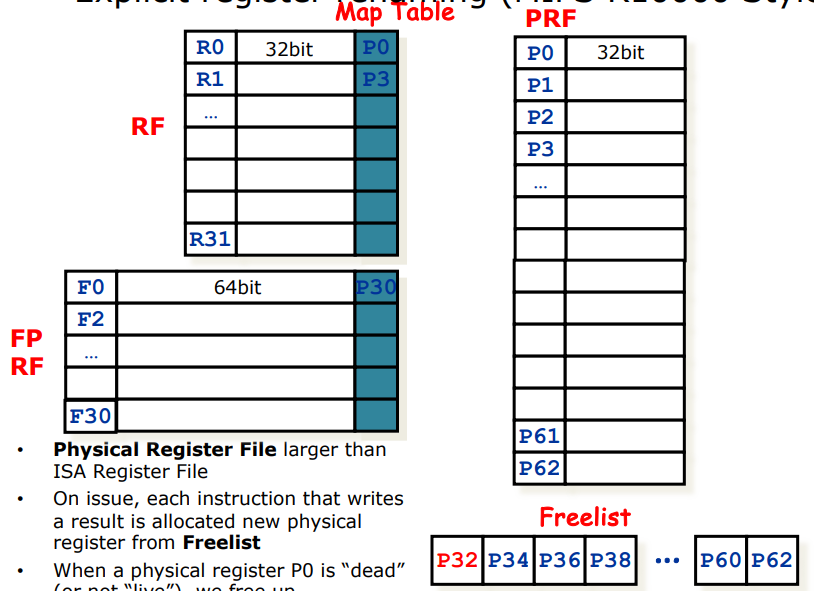
\includegraphics[width=0.4\linewidth]{images/err.png}
    \caption{Explicit register renaming}
\end{figure}
Expanding the Physical Register File beyond the size of the Instruction Set Architecture (ISA) Register File involves several steps:
\begin{enumerate}
    \item Upon issuance, every instruction that generates a result is assigned a new physical register from the available free list.
    \item  When a physical register, denoted as P0, is no longer in use (i.e., it becomes "dead" or not "live"), it is released back to the free list for future allocations.
\end{enumerate}
Explicit Register Renaming involves maintaining a translation table that maps ISA registers to physical registers. 
When an instruction writes to a register, its corresponding entry in the translation table is updated with a new register from the available pool. 
Physical registers are released when they are no longer utilized by any active instructions.
\begin{figure}[H]
    \centering
    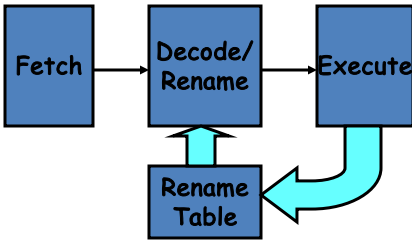
\includegraphics[width=0.4\linewidth]{images/errm.png}
    \caption{Explicit register renaming mechanism}
\end{figure}

\paragraph*{Unified physical register file}
In the Unified Physical Register File approach, architectural registers are unified into a single physical register file during the decoding stage, without reading register values. 
Functional units interact with this unified register file, accessing and updating both committed and temporary registers during execution. 
The process of committing involves updating the mapping of architectural registers to physical registers without moving any data.
\begin{figure}[H]
    \centering
    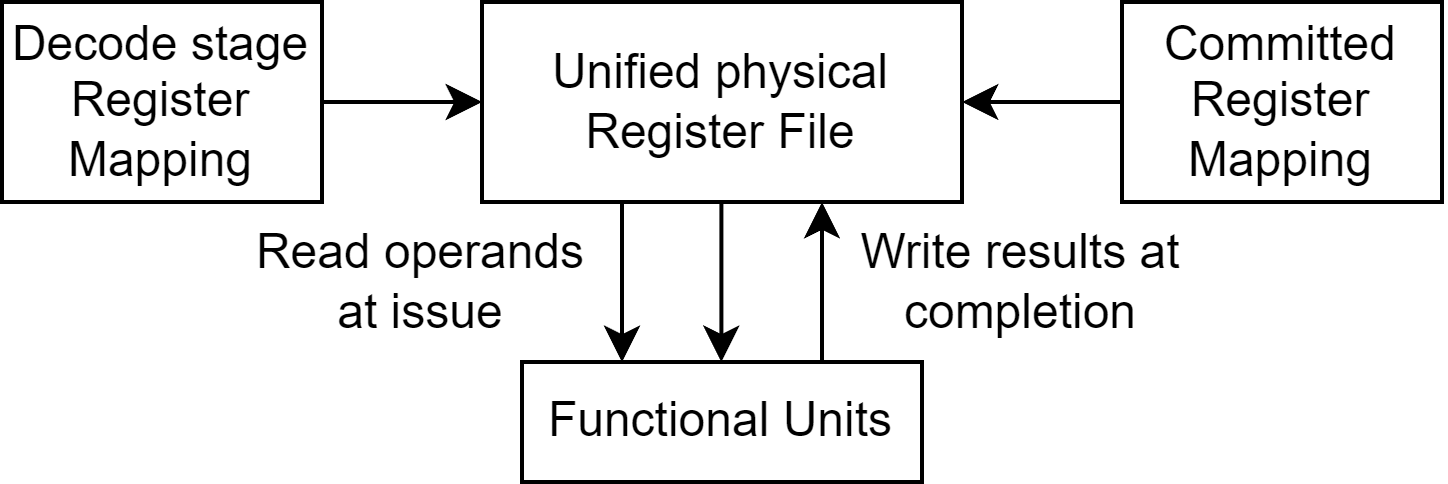
\includegraphics[width=0.4\linewidth]{images/uprf.png}
    \caption{Unified Physical Register File}
\end{figure}

\paragraph*{Instruction commit}
Instruction Commit involves several steps:
\begin{itemize}
    \item It marks the mapping between an architectural register number and a physical register number as non-speculative, indicating that it's finalized.
    \item It releases any physical registers used to store the previous value of the architectural register.
    \item Deallocating registers is a bit complex:
        \begin{itemize}
            \item Before freeing a physical register, it's necessary to ensure it no longer corresponds to an architectural register and there are no further outstanding uses of it.
            \item A physical register remains associated with an architectural register until that register is overwritten.
            \item However, there might still be outstanding uses of the physical register. The processor checks if any source operand in the functional units queue corresponds to that register. If not, it can be deallocated.
        \end{itemize}
        Alternatively, the processor can wait until another instruction that writes to the same architectural register commits. This method may slightly prolong the usage of a physical register but is easier to implement.
\end{itemize}

\subsection{Hardware register renaming}
To perform hardware register renaming, the following components are necessary:
\begin{itemize}
    \item \textit{Renaming map}: this is a simple data structure that provides the physical register number corresponding to the requested architectural register.
    \item \textit{Instruction commit}: this process involves permanently updating the renaming table to indicate that the physical register holding the destination value corresponds to the actual architectural register.
\end{itemize}
Using a ReOrder Buffer (ROB) enforces in-order commit.
Use ROB to enforce in-order commit
\begin{figure}[H]
    \centering
    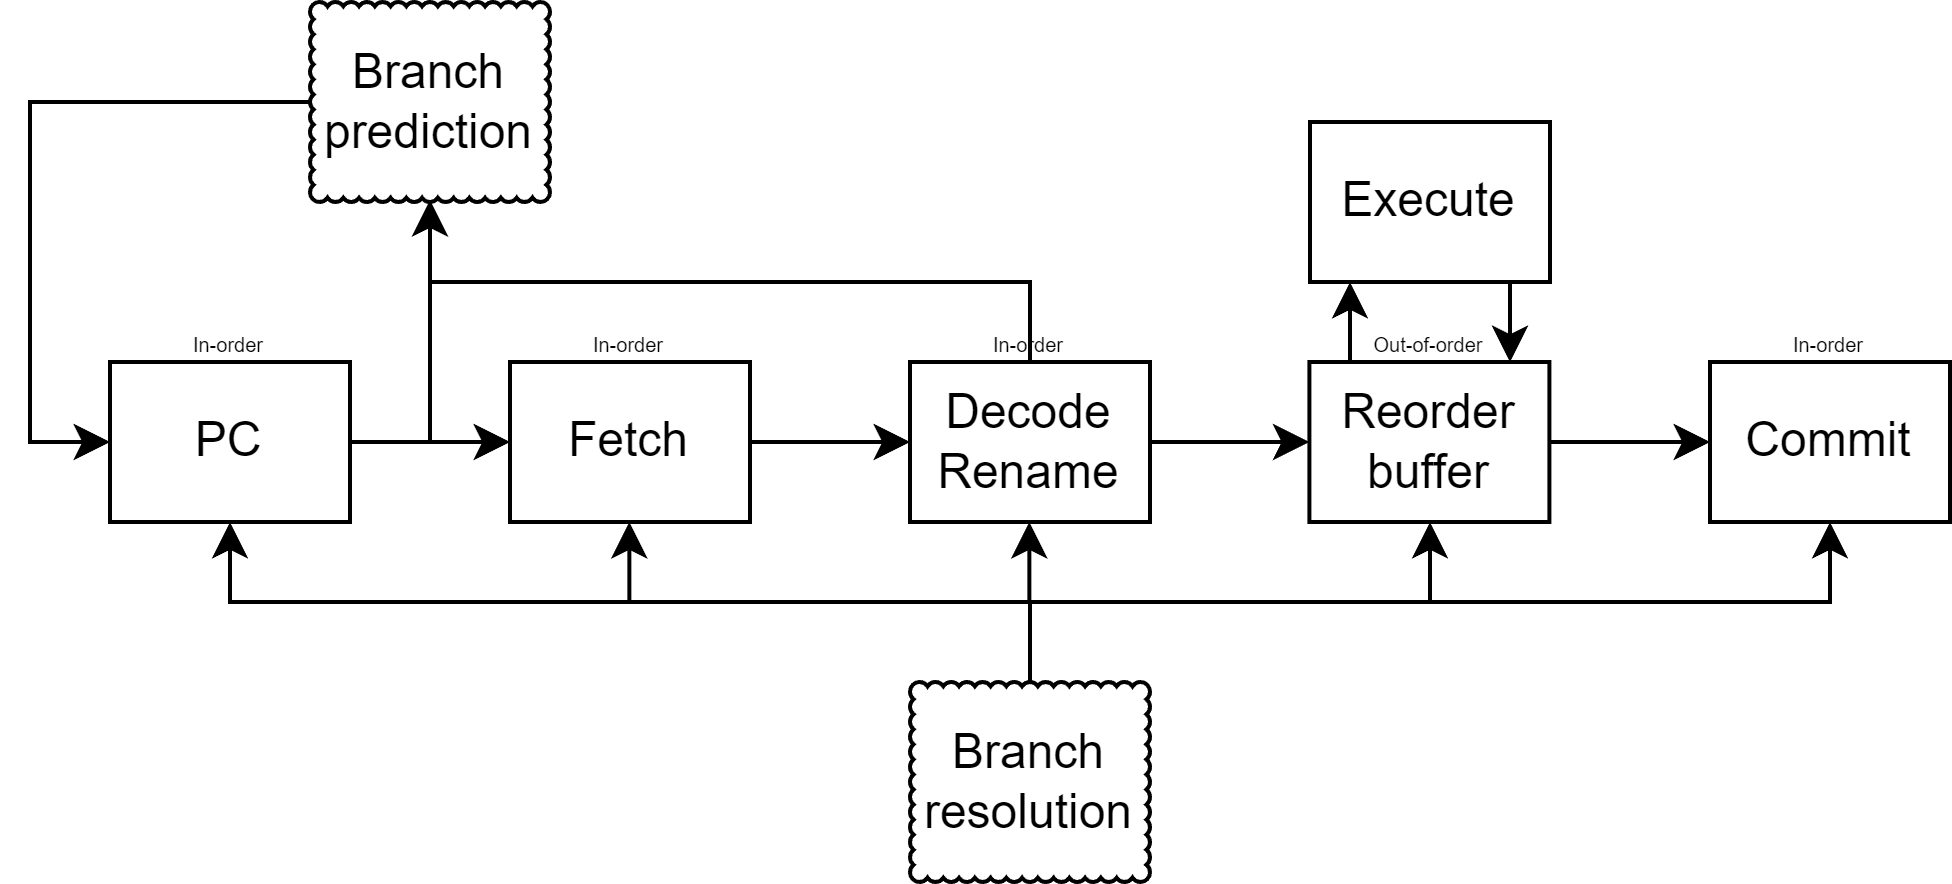
\includegraphics[width=0.4\linewidth]{images/herr.png}
    \caption{Hardware explicit register renaming}
\end{figure}

\paragraph*{Advantages}
The main advantages include:
\begin{itemize}
    \item \textit{Decoupling renaming from scheduling}: this approach allows for flexibility in pipeline design. 
        The pipeline can resemble a standard DLX pipeline with the possibility of issuing multiple operations per cycle. 
        Alternatively, it could adopt methodologies like Tomasulo's algorithm or scoreboard-based approaches. 
        Standard forwarding or bypassing techniques can be employed.
    \item \textit{Single register file access}: data retrieval from a single register file is facilitated. 
        This eliminates the need to bypass values from the reorder buffer, which can be crucial for maintaining pipeline balance.
    \item \textit{Widespread adoption}: many processors have adopted variants of this technique, including the R10000, Alpha 21264, and HP PA8000 processors.
\end{itemize}

\paragraph*{Support}
Ensuring swift access to a translation table involves deploying a physical register file with a capacity exceeding that specified by the Instruction Set Architecture (ISA).
This setup enables quick determination of available physical registers, crucial for seamless operation. 
In instances where no registers are available, the system pauses during instruction issuance. 
Consequently, reservation stations are unnecessary for register renaming. 
However, many modern architectures combine explicit register renaming with Tomasulo-like reservation stations to effectively control execution flow.

\subsection{Explicit register renaming and scoreboard}
Explicit Register Renaming involves using a physical register file that surpasses the number of registers specified by the ISA. 
Here's how it works:
\begin{itemize}
    \item \textit{Translation table}: a translation table maintains the mapping between ISA registers and physical registers. 
        When a register is written to, its entry in the table is updated with a new register from the free list. 
        Physical registers are marked as free when not in use by any active instructions.
    \item \textit{Pipeline structure}: the pipeline structure can mirror a standard DLX pipeline with stages like Instruction Fetch (IF), Instruction Decode (ID), Execute (EX), etc. 
\end{itemize}
The advantages are: 
\begin{itemize}
    \item Eliminates Write-After-Read (WAR) and Write-After-Write (WAW) hazards.
    \item Facilitates full out-of-order completion similar to Tomasulo's approach.
    \item Simplifies architectural design by enabling data retrieval from a single register file.
    \item Simplifies speculative execution and precise interrupt handling: only requires undoing the table mappings for precise breakpoint restoration.
\end{itemize}

Scoreboard Control Stages with Explicit Renaming:
\begin{enumerate}
    \item \textit{Issue}: decode instructions, check for structural hazards, and allocate new physical registers for results. Instructions are issued in program order for hazard checking. Issuance is withheld if there are no free physical registers or if there's a structural hazard.
    \item \textit{Read operands}: wait until no hazards, then read operands. All real dependencies (RAW hazards) are resolved in this stage since it waits for instructions to write back data.
    \item \textit{Execution}: functional units begin execution upon receiving operands. When the result is ready, it notifies the scoreboard.
    \item \textit{Write result}: execution finishes, and results are written.
\end{enumerate}
Note that there are no checks for WAR or WAW hazards in this approach.

\paragraph*{Register renaming and ROB}
When contrasting Register Renaming with ReOrder Buffer:
\begin{itemize}
    \item Committing instructions is simpler in Register Renaming compared to ROB.
    \item However, deallocating registers poses more complexity in Register Renaming.
    \item The dynamic mapping of architectural to physical registers adds intricacy to the design and debugging processes.
    \item Register Renaming is employed in several architectures such as PowerPC603/604, Pentium II-III-4, MIPS 10000/12000, Alpha 21264, and Sandy-Bridge. 
        These architectures typically incorporate an additional 20 to 80 registers.
\end{itemize}

\subsection{Summary}
In Explicit Renaming, there are more physical registers available than needed by the ISA.
Here's a breakdown:
\begin{itemize}
    \item \textit{Rename table}: this keeps track of the current association between architectural registers and physical registers.
    \item \textit{Translation table}: used to perform compiler-like transformations on-the-fly.
\end{itemize}
With Explicit Renaming:
\begin{itemize}
    \item All registers are concentrated in a single register file.
    \item It allows for the utilization of a bypass network that resembles a 5-stage pipeline.
    \item Introduces a register-allocation problem that needs to be managed.
    \item Handling branch misprediction and precise exceptions differs from other methods, but ultimately simplifies processes.
    \item For precise exceptions and branch prediction, a mechanism like a reorder buffer is essential.
\end{itemize}

\paragraph*{Multiple issue}
To handle multiple instructions simultaneously, including potential dependencies between them, is crucial for dynamically scheduled superscalar processors. 
This capability represents one of the fundamental bottlenecks in their design:
\begin{itemize}
    \item \textit{Issue logic complexity}: designing logic to manage all possible combinations of dependent instructions within a single clock cycle is challenging. 
        As the number of instructions issued per cycle increases, the complexity grows exponentially.
    \item \textit{Basic strategy}: 
        \begin{itemize}
            \item Assign a reservation station and a reorder buffer entry for each instruction in the next issue bundle. 
                If unavailable, only a subset of instructions is considered sequentially.
            \item Analyze all dependencies among the instructions.
            \item Update the reservation table for dependent instructions using the assigned reorder buffer number if an instruction in the bundle relies on an earlier one within the same bundle.
        \end{itemize}
\end{itemize}
This process is executed in parallel within a single clock cycle. 
Additionally, the ability to commit multiple instructions in one clock cycle is essential. 
Intel I7 processors employ a similar technique.

Multiple Instructions Issue with Register Renaming:
\begin{itemize}
    \item The issue logic pre-reserves adequate physical registers for the entire issue bundle.
    \item It identifies dependencies within the bundle:
        \begin{itemize}
            \item If no dependence exists within the bundle, the register renaming structure determines the physical register holding or will hold the required result from an earlier issue bundle.
            \item If an instruction depends on an earlier one within the bundle, the pre-reserved physical register for the result is used to update the issuing instruction's information.
        \end{itemize}
\end{itemize}
Again, all these operations are conducted simultaneously in a single clock cycle.

\paragraph*{Superscalar Register Renaming: two-issue}
In the context of Superscalar Register Renaming with a two-issue capability:
\begin{itemize}
    \item Allocation during decode: instructions are assigned new physical destination registers.
    \item Operand renaming: source operands are renamed to the physical register holding the most recent value.
    \item Execution unit view: execution units exclusively utilize physical register numbers.
    \item Hazard checking: it's imperative to inspect for Read-After-Write (RAW) hazards between instructions issuing in the same cycle. 
        This verification can be conducted concurrently with the rename lookup process.
\end{itemize}

\paragraph*{Speculation and energy efficiency}
Speculation tends to elevate power consumption while reducing execution time to a greater extent, ultimately resulting in overall energy savings. 
The total energy consumed may decrease depending on the number of incorrectly executed instructions. 
Empirical findings indicate that misspeculation in scientific code is generally minimal, whereas it can be more substantial, averaging around 30\%, in integer code.

\paragraph*{Summary}
Modern computer architects employ extensive prediction techniques for branches, data dependencies, and data access. 
While predicting branches can be achieved with relatively simple hardware structures such as the Branch Target Buffer (BTB) and Branch History Table (BHT), more sophisticated prediction methods like correlation are also utilized to handle interdependent branches.

Explicit Register Renaming involves employing more physical registers than specified by the ISA. 
This approach decouples renaming from scheduling, offering flexibility in resolving Read-After-Write (RAW) hazards. 
It relies on a rename table to track the current association between architectural and physical registers, although managing this table can be complex.

However, achieving parallelism efficiently from real hardware remains challenging despite these advancements.